\documentclass[12pt]{report}
\usepackage[margin=0.5in]{geometry}
\usepackage[fleqn]{amsmath}
\usepackage{nccmath}
\usepackage{alltt}
\usepackage{sectsty}
\usepackage{titlesec}
\newcommand{\ts}{\textsuperscript}
\usepackage{graphicx}
\graphicspath{ {../images/} }
\usepackage{subfig}


\titlespacing*{\section}{0pt}{0.8\baselineskip}{0.2\baselineskip}

\begin{document}

\begin{titlepage}
    \begin{center}
        \vspace*{1cm}
        
        \textbf{CO3093 COURSEWORK 1 Report}
        
        \vspace{0.5cm}
		Big Data \& Predictive Analytics - Simulation-based \& Regression Models
        
        \vspace{1.5cm}
        
        \textbf{Ihtasham Chaudhry}
        
        \vfill
        
        \vspace{0.8cm}
                
        Department of Informatics\\
        University of Leicester\\
        23\ts{rd} February 2018
        
    \end{center}
\end{titlepage}

\newpage

\section{Question 1}

\vspace{0.5cm}

\subsection{1.1}

\vspace{0.5cm}

It is important to consider missing values in our data set and to filter out the columns based on this information so that we have all the information we need to make predictions and have \emph{clean} data. In the case of our problem (predicting a winner), the most important factors that we must consider are win/loss statistics and goals scored/conceded statistics.

\noindent
We can then draw some conclusions from the data such as:
\begin{enumerate}
	\item The average number of goals scored per match throughout the tournament by each team playing at home is 1.49 and away is 1.18. We also notice that the median of these values falls close to the minimum values which indicates that the data on this column is positively skewed and has a longer tail towards higher values.
	\item From this data we can also observe that on average teams win more games playing home than they do playing away, The mean ($\mu$) of wins at home for each team is larger than the median of the dataset, this indicates that the distribution is skewed towards large values. The standard deviation ($\sigma$) is very small relative to the min and max values, this indicates that the distribution has "long tails". 
	 \item Following from the previous point, the same observation can be made regarding the number of "FTHG" or "Full Time Home Goals" by each team per match. The data again is skewed towards larger values. 
	 
\end{enumerate}

\subsection{1.2}
\noindent
As we are only considering two teams; Manchester United and Manchester City, we can further filter the data and extract only the games played by both of those teams where they are playing either home or away. When we accumulate the data by teams and their home and away games to see how they perform for each category. After doing this we can draw some analysis from the data.

\vspace{0.3cm}
\noindent

\iffalse
\begin{table}[ht]
\centering
\caption{Full time results over the season (higher is better)}
\begin{tabular}{lllll}
         & Wins & Losses & Draws &  \\
Man Utd  & 16 & 3 &  5 & \\
Man City & 21 & 1 & 2 &\\

\end{tabular}
\end{table}
\fi

\begin{table}[ht]
\centering
\caption{Mean goals scored per game over the season (higher is better)}
\begin{tabular}{lllll}
         & Home & Away &  &  \\
Man Utd  & 2.25 & 1.83 &  &  \\
Man City & 3.50 & 2.33 &  &  \\
\end{tabular}
\end{table}

\begin{table}[ht]
\centering
\caption{Mean goals conceded per game over the season (lower is better)}
\begin{tabular}{lllll}
         & Home & Away &  &  \\
Man Utd  & 0.41 & 0.91 &  &  \\
Man City & 0.75 & 0.75 &  &  \\
\end{tabular}
\end{table}

\noindent
We can see that over 24 games played by both teams over the course of the season, Man City has a higher average of goals both in the home and away side compared to Manchester United, and have conceded a higher average of goals home but a lesser average of goals home compared to Manchester United. 

\newpage

\subsection{1.3}
\vspace{0.3cm}
We can visualise this information and compare the offensive and defensive performance of the two teams. To do this we will consider goal scores. To measure the defensive performance of a team we can see how many goals were conceded by the team playing home, lower is better in this case, i.e we want to see that the distribution is skewed towards less goals. And in contrast to this to measure offensive performance we can see how many goals they scored away, higher is better in this case and alternatively we want to see that the data is skewed more towards the right to see which is the better team. 

\begin{figure}[ht]
  \centering
      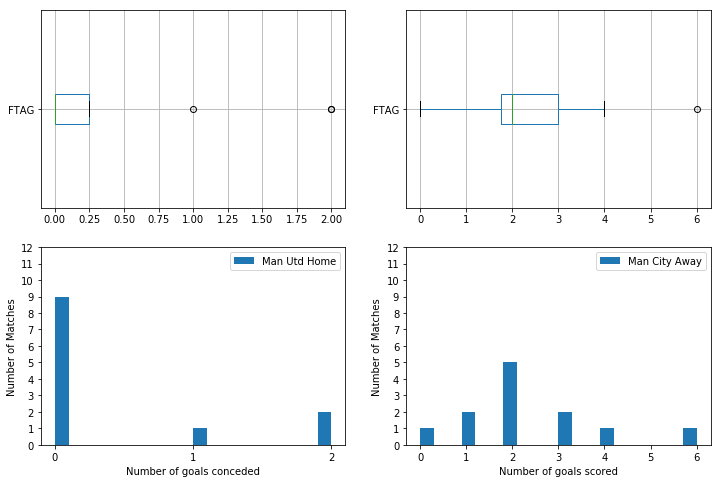
\includegraphics[width=1\textwidth]{fig1}
  \caption{A comparison of M.U's Home defence against M.C's away offence.}
\end{figure}
\vspace{0.3cm}

From this graph we can see that Manchester United's defence is quite strong, this is because out of 12 games playing at home they only conceded goals in 3 out of those 12 games. Furthermore, we can also see that Manchester City's offence is fairly strong and we can tell that the number of goals they score on the away side is almost distributed in a Poisson distribution manner. From the boxplots we can see that Manchester City's goals away were between 2 and 3. 

\newpage
\begin{figure}[ht]
  \centering
      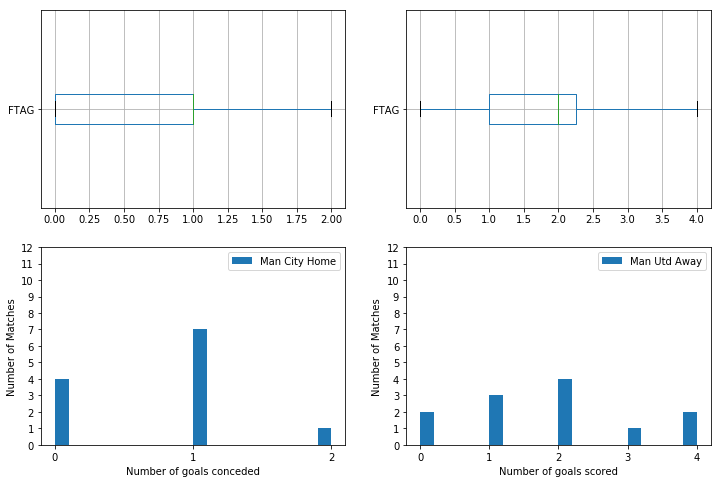
\includegraphics[width=1\textwidth]{fig2}
  \caption{A comparison of M.C's Home defence against M.C's away offence.}
\end{figure}
\vspace{0.3cm}

In contrast to the above graph, we can see that Manchester City's home defence is worse than Manchester United's home defence. We can assert this by seeing that Manchester City conceded at least 1 goal in 8 matches compared to the 3 that Manchester United conceded at home. Furthermore, we can also see that Manchester United's goals scored away are more spread out and have a higher mean than Man City's. However we can also see that at most Man Utd only scored 4 goals in any one game over the whole season compared to the 6 scored by Man City which could indicate a higher level of offence. 

\subsection{Simulation}
\vspace{0.3cm}

To simulate the matches between Manchester United and Manchester City we can use a Poisson distribution model because it concerns a discrete probability distribution which is relevant to the case of football matches. Furthermore, in our model we also consider that each event or match is independent from each other.

\vspace{0.3cm}
\noindent
By using this we can generate scores between the two teams based on the historical data of the two teams and create paired random drawings. It is obvious that the higher number of fantasy games we create, the more accurate our model will be able to predict as a higher sample size means that we have more confidence in our prediction. In this case we will generate 10000 matches per side for each team, i.e. 1000 games where MU plays home, 1000 games where MU plays away and the same for MC. After pairing these results we will get 1000 games played by each team on the home side and away side resulting in a total of 2000 simulated fantasy games. After running this simulation, we may get the following result.

\newpage
\begin{table}[ht]
\centering
\caption{Wins for each team and the side they played on}
\begin{tabular}{lllll}
         & MC Win & MU Win &  &  \\
Home  & 691 & 386 &  &  \\
Away & 427 & 174 &  &  \\
\end{tabular}
\end{table}

\vspace{0.3cm}
\noindent
And we can also consider the number of times the teams drawed against each other which in this case was: \textbf{322}.

\vspace{0.3cm}

We can then find the probability of who will win the match based on the simulation from the fantasy games we've generated. In the most basic finding we can simply find out the probability of a team winning a match. For this we can observe the following probabilities:
\begin{equation*}
	\begin{aligned}
    	& P(ManUtdWin) \\ 
    	& P(ManCityWin) \\
    	& P(Draw)
	\end{aligned}
\end{equation*}
\noindent
After calculating these probabilities we get the following results:

\vspace{0.3cm}
\noindent
\begin{equation*}
	\begin{aligned}
    	& P(ManUtdWin) = \textbf{0.2845} \\ 
    	& P(ManCityWin) = \textbf{0.5585} \\
    	& P(Draw) = \textbf{0.157}
	\end{aligned}
\end{equation*}

\vspace{0.3cm}
\noindent
Here we can see that Manchester City has a much larger chance of winning the game based on the simulations we've done and even looking at the data from the premier league it is obvious that Manchester City was the better team. However, to break down these results we can also observe the following probabilities to give us a better outlook into the chances of winning for each team:

\vspace{0.3cm}
\noindent
\begin{equation*}
	\begin{aligned}
    	& P(ManUnitedWin \mid Home) = \textbf{0.492}\\ 
    	& P(ManUnitedWin \mid Away) = \textbf{0.194}\\
    	& P(ManCityWin \mid Home) = \textbf{0.806}\\
    	& P(ManCityWin \mid Away) = \textbf{0.508}	
	\end{aligned}
\end{equation*}

\vspace{0.3cm}
\noindent
From this we can observe that Manchester City has a higher chance of winning both playing home or away compared to Manchester United. From this we can confidently predict that in a match up of Manchester United vs Manchester City in the Premier League, based on the historical data; Manchester City will win the game.

\noindent\rule{2cm}{0.4pt}

\vspace{0.3cm}
\noindent
\textbf{Verifying our model} 

\noindent
To test our simulation further, we can observe the scores for another team and try to predict what results we can obtain. For an example let us take Chelsea vs Arsenal as a candidate match-up. We can see that in the premier league, the following scores were observed between the two teams:

\vspace{0.3cm}

\begin{table}[ht]
\centering
\caption{Matchups between Chelsea and Arsenal in the BPL}
\label{t4}
\begin{tabular}{lllll}
Home Team & Away Team & FTHG & FTAG & Winner \\
Chelsea   & Arsenal   & 0    & 0    & Draw   \\
Arsenal   & Chelsea   & 2    & 2    & Draw  
\end{tabular}
\end{table}

\clearpage
Here we can see that these teams drew in both their games together, but we can look a little bit further into their mean goals scored per game over the premier league per match:

\vspace{0.3cm}

\begin{table}[ht]
\centering
\caption{Mean goals scored per match}
\label{t5}
\begin{tabular}{lll}
        & Mean goals home & Mean goals away \\
Chelsea & 1.75            & 2.00            \\
Arsenal & 2.58            & 1.67           
\end{tabular}
\end{table}

Here we can see that Chelsea has a better chance of scoring more goals if they're playing away and Arsenal has a higher chance of scoring more goals if they're playing home. We can now generate a small number of matches with these teams and stack them up against each other to see how our simulation performs.

\vspace{0.3cm}
\noindent
After creating fantasy games between Chelsea and Arsenal based on our simulation model we get the following results:

\begin{table}[ht]
\centering
\caption{Number of wins by each team}
\label{t6}
\begin{tabular}{lll}
        & Wins at Home & Wins Away \\
Chelsea & 4            & 3         \\
Arsenal & 7            & 1        
\end{tabular}
\end{table}

\noindent
Addition to this data, there was a total of 5 draws between the teams. Looking over the data in Table 5 we can verify that these are feasible predictions by our models. Thus we can conclude that our model is very likely perform accurately when predicting a winner.  

\newpage
\section{Question 2}
\subsection{2.1}

From the provided csv file we can generate a time-series using the "adjusted close" column and plot the data. After doing this we obtain the following figures:

\begin{figure}[!htbp]
    \centering
    \subfloat[Time series of Apple Stock closing prices from 1980 to 2018]{{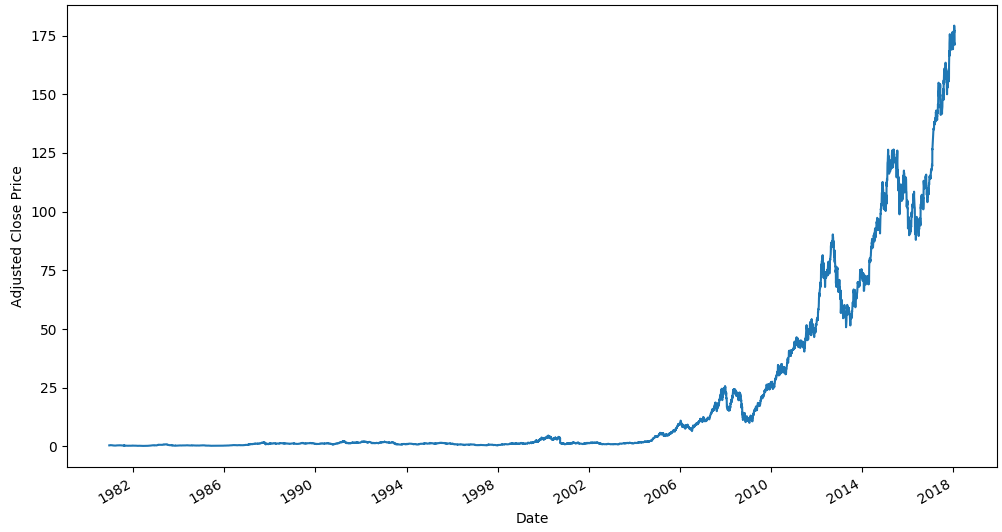
\includegraphics[width=0.9\textwidth]{fig3} }}%
    \qquad
    \subfloat[Time series of Apple Stock closing prices from 2007 to 2018]{{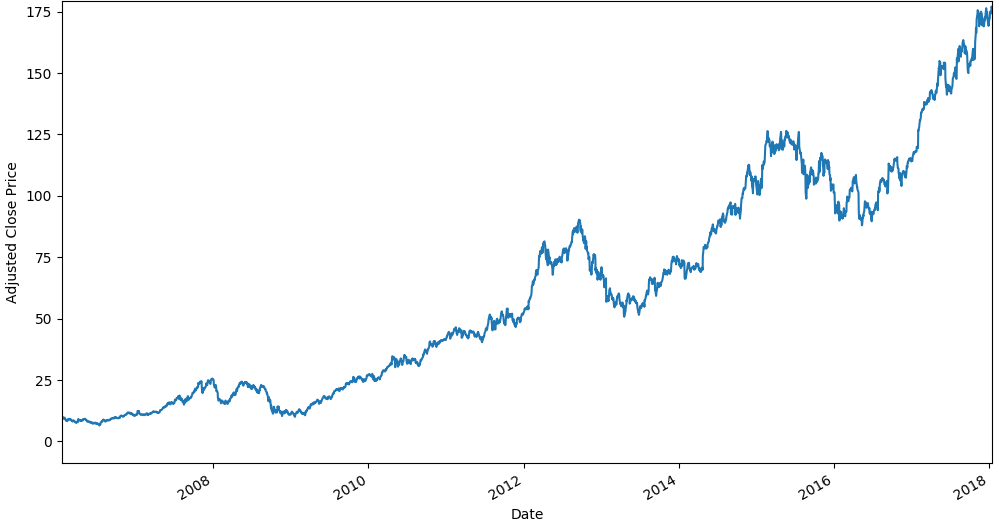
\includegraphics[width=0.9\textwidth]{fig4} }}%
    \caption{Time series of the Apple stock prices with different time ranges}%
    \label{fig:example}%
\end{figure}

\newpage
\noindent
By observing Figure 3 we can make the following analyses:

\begin{enumerate}
	\item Up until 2004 the stock price was very low and remained low, there were no peaks or changes in the price.
	\item From 2005/2006 the stock prices started rising at an exponential rate, peaking in 2012 at \$90.30. An then started to heavily decline thereafter.
	\item The stock prices then started to rise between 2013 and 2015 where they peaked and started to fall once again and the same trend occurred between the years of 2016 and 2018. 
	\item Overall we can also see that from 2006 to 2018, in the matter of 12 years the stock prices have multiplied by roughly 16 times, which shows that Apple has been a very successful company. 
	\item Though the prices have increased in this time period, we can also observe that the prices have been very unstable and there seems to be a trend of prices increasing all year round and then falling the beginning of the next annual year. Upon close inspection of the prices this becomes more clear. This can be seen in Figure 3(b). However it is still evident that the prices are generally inclining each year. 
\end{enumerate}

\section{2.2}

The model that we will mainly be concerned with is the Multiple Linear Regression model where we have more than one predictor. The reason for this is because we have more than one attribute that may help us predict an output. In essence we will be able to create a linear function based on predictors which will model like the following:

\begin{equation*}
	f(x_{i}) = b_{0} + b_{1}x_{i,1} + b_{2}x_{i,2} + b_{n}x_{i,n}
\end{equation*}



\newpage

\end{document}